%\documentstyle[10pt,twoside]{article}
%\documentstyle[twoside]{article}
\documentclass[twoside]{article}
\setlength{\oddsidemargin}{0.25 in}
\setlength{\evensidemargin}{-0.25 in}
\setlength{\topmargin}{-0.6 in}
\setlength{\textwidth}{6.5 in}
\setlength{\textheight}{8.5 in}
\setlength{\headsep}{0.75 in}
\setlength{\parindent}{0 in}
\setlength{\parskip}{0.1 in}

\usepackage{graphicx}
\usepackage{url}
\usepackage{pdfpages}

%
% The following commands sets up the lecnum (lecture number)
% counter and make various numbering schemes work relative
% to the lecture number.
%
\newcounter{lecnum}
\renewcommand{\thepage}{\thelecnum-\arabic{page}}
\renewcommand{\thesection}{\thelecnum.\arabic{section}}
\renewcommand{\theequation}{\thelecnum.\arabic{equation}}
\renewcommand{\thefigure}{\thelecnum.\arabic{figure}}
\renewcommand{\thetable}{\thelecnum.\arabic{table}}
\newcommand{\dnl}{\mbox{}\par}

%
% The following macro is used to generate the header.
%
\newcommand{\lecture}[4]{
   \pagestyle{myheadings}
   \thispagestyle{plain}
   \newpage
   \setcounter{lecnum}{#1}
   \setcounter{page}{1}
   \noindent
   \begin{center}
   \framebox{
      \vbox{\vspace{2mm}
    \hbox to 6.28in { {\bf CMPSCI~677~~~Operating Systems
                        \hfill Spring 2019} }
       \vspace{4mm}
       \hbox to 6.28in { {\Large \hfill Lecture #1: #2  \hfill} }
       \vspace{2mm}
       \hbox to 6.28in { {\it Lecturer: #3 \hfill Scribe: #4} }
      \vspace{2mm}}
   }
   \end{center}
   \markboth{Lecture #1: #2}{Lecture #1: #2}
   \vspace*{4mm}
}

%
% Convention for citations is authors' initials followed by the year.
% For example, to cite a paper by Leighton and Maggs you would type
% \cite{LM89}, and to cite a paper by Strassen you would type \cite{S69}.
% (To avoid bibliography problems, for now we redefine the \cite command.)
%
\renewcommand{\cite}[1]{[#1]}

% \input{epsf}

%Use this command for a figure; it puts a figure in wherever you want it.
%usage: \fig{NUMBER}{FIGURE-SIZE}{CAPTION}{FILENAME}
\newcommand{\fig}[4]{
            %\vspace{0.2 in}
            \centerline{\includegraphics[scale=#2]{#4}}
            \begin{center}
            Figure \thelecnum.#1:~#3
            \end{center}
    }

% Use these for theorems, lemmas, proofs, etc.
\newtheorem{theorem}{Theorem}[lecnum]
\newtheorem{lemma}[theorem]{Lemma}
\newtheorem{proposition}[theorem]{Proposition}
\newtheorem{claim}[theorem]{Claim}
\newtheorem{corollary}[theorem]{Corollary}
\newtheorem{definition}[theorem]{Definition}
\newenvironment{proof}{{\bf Proof:}}{\hfill\rule{2mm}{2mm}}

% Some useful equation alignment commands, borrowed from TeX
\makeatletter
\def\eqalign#1{\,\vcenter{\openup\jot\m@th
  \ialign{\strut\hfil$\displaystyle{##}$&$\displaystyle{{}##}$\hfil
      \crcr#1\crcr}}\,}
\def\eqalignno#1{\displ@y \tabskip\@centering
  \halign to\displaywidth{\hfil$\displaystyle{##}$\tabskip\z@skip
    &$\displaystyle{{}##}$\hfil\tabskip\@centering
    &\llap{$##$}\tabskip\z@skip\crcr
    #1\crcr}}
\def\leqalignno#1{\displ@y \tabskip\@centering
  \halign to\displaywidth{\hfil$\displaystyle{##}$\tabskip\z@skip
    &$\displaystyle{{}##}$\hfil\tabskip\@centering
    &\kern-\displaywidth\rlap{$##$}\tabskip\displaywidth\crcr
    #1\crcr}}
\makeatother

% **** IF YOU WANT TO DEFINE ADDITIONAL MACROS FOR YOURSELF, PUT THEM HERE:



% Some general latex examples and examples making use of the
% macros follow.

\begin{document}

%FILL IN THE RIGHT INFO.
%\lecture{**LECTURE-NUMBER**}{**DATE**}{**LECTURER**}{**SCRIBE**}
\lecture{8}{February 14}{Prashant Shenoy }{\textbf{Ashish Ranjan}}

%\section{Virtual Machine Migration (Continued)}

%\begin{itemize}
  %\item \textbf{Post-copy VM Migration} : In this method, the virtual CPU state is copied to the destination prior to copying the memory state. Execution is started right-away and then the memory state is copied. During execution, if any memory access results in access to a part of memory that has not been copied yet, it is resolved over network. Migration is complete when memory state has been copied completely. Post-copy migration achieves immediacy of migration by trading it with performance.
%\end{itemize}

%\begin{figure}[h]
%\centering
%\includegraphics[scale=0.75]{pre_post_copy.pdf}
%\caption{Pre-copy vs Post-copy}
%\end{figure}

\section{Communication in distributed systems}

In a distributed system, each entity may want to share information with other distributed entities. For example, a temperature sensor may want to share its information with a climate control system. The processes run on different machines and the applications implemented by these processes might include communication between them.

\subsection{Types of communication in distributed systems}
Communication among distributed processes can be categorized into:\\
\textbf{1. Unstructured communication} - It involves using memory buffers to pass information between the processes. So you might have a shared memory region on a machine. Process can read and write to that shared memory region and then some other prcoess can use that information. uses shared memory or shared data structures; Update a distributed shared memory to let others know of your local state. Others can then read the distributed shared memory to get your local state. No explicit messages are used.\\
\textbf{2. Structured communication} - also called as 'message passing', this uses explicit messages (or inter-process communication mechanisms) over network. There is no shared memory in this type of communication. The processes can be on same machines or different machines.

\subsection{Distributed communication protocols}
\begin{description}
\item{ \textbf{Communication Protocols}} : Protocols are a set of rules for communication agreed by all the entities participating in communication. Protocols can be connection oriented (TCP) or connectionless (UDP). In a layered network model, when a message is sent over network, each layer adds its own header and trailer information. (In brief:\textbf{Physical layer} corresponds to the actual transmission of bits on Network [using WiFi/cable], in other words it says what is the medium of communication; \textbf{Data Link or MAC layer} decides format of the message, creates 'frames' and passes down; \textbf{Network Layer} is involved in hop by hop communication and all the routing mechanisms come into play here. In TCP/IP protocol stack, the IP layer is the network layer; \textbf{Transport Layer} usually is end to end communication. Flow and error control [as in TCP] are present here); \textbf{Session Layer} looks at the user session; \textbf{Presentation Layer} looks at how is the data presented to the application; \textbf{Application Layer} Things like HTTP, FTP which are applications using this protocol stack for comunication.)
\\\textbf{Q: So are the arrows in the Communication Protocol figure wrong?}\\
{Instructor: The arrows are taken from the book. But in reality one set of arrows go down the stack and another up the stack}
\\\textbf{Q: Can you do unstructured communication if processes are on a different machines?}\\
{Instructor: I gave you the example of shared memory. You can have processes on different machines. But in that case the shared memory region has to be network accesible. Example keep a file on file server. Process A writes to that file and Process B on some other machine reads that file. Because file server shares files across machines, you can have unstructured communication. You can also have distributed shared memories shared across machines but it is more complex.}
\item{ \textbf{Middleware Protocols}} : Middleware layer resides between an application and the operating system. Middleware layer may implement its own general purpose protocol that may even result in more layers. Example: Distributed system. As part of this course, we deal a lot, with this Middleware layer.
\begin{figure}[h]
\centering
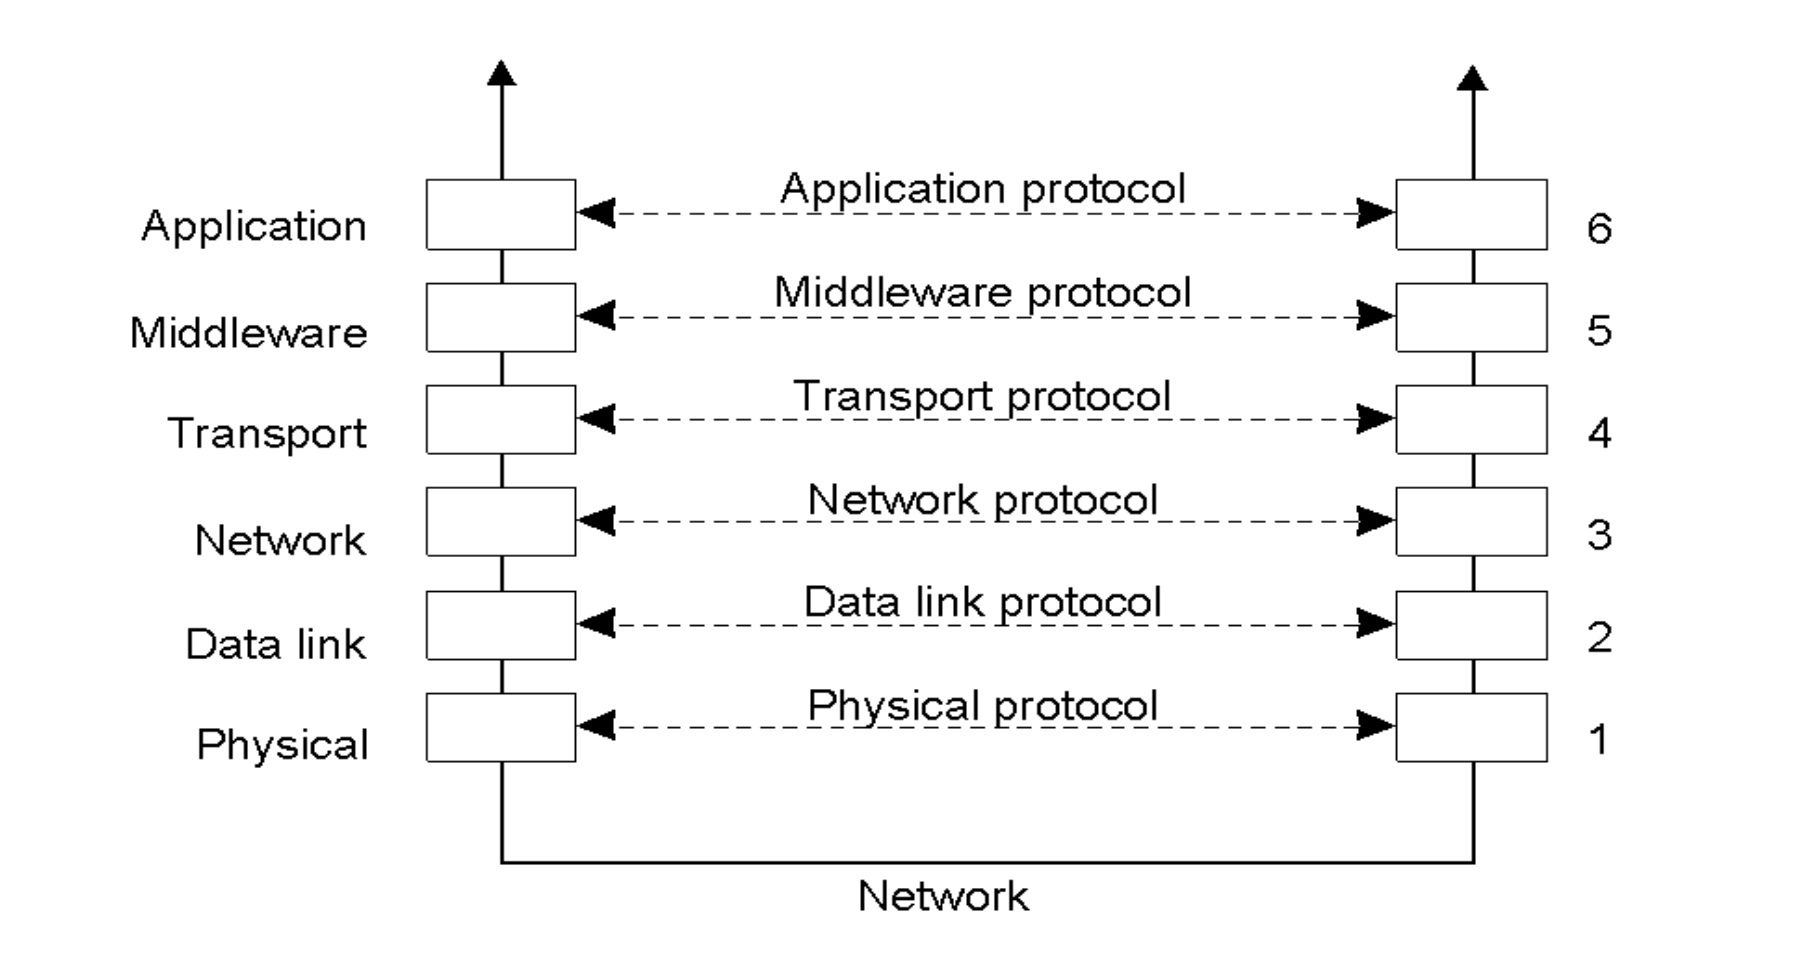
\includegraphics[scale=0.5]{layers.png}
\caption{Middleware protocol}
\end{figure}
\begin{figure}[h]
\centering
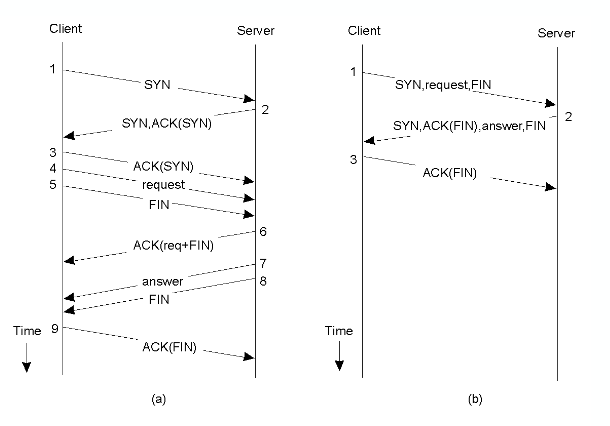
\includegraphics[scale=0.75]{client_server_tcp.png}
\caption{TCP connection}
\end{figure}
\item{\textbf{Client - Server using TCP}} : In a standard TCP communication, for just a single request from client we need almost 9 packets (and that too assuming there are no losses) in order to exchange the two real messages. In a TCP connection, every packet needs to be acknowledged (the message 4 which was the request and message 7 which was the answer that came back from the server as shown in Figure 8.2 (a)). Also note that TCP does not have to acknowledge every single message, it can acknowledge a batch of messages. Figure 8.2 (a) shows this in detail (along with the customary 3-way handshake to initiate the connection or tear it down). To make this process efficient (especially for short request scenarios from client side, as above) mechanisms like grouping do exist (Figure 8.2 (b)).
\\\textbf{Q: The figure 8.2(b) seems like a better method. Why is it not used?}\\
{Instructor: This method is not a general purpose protocol. It works good for short request scenarios. So you have to take care of different scenarios. It might work for one scenario, might not work for the other. If you see TCP, that is a general purpose protocol.}
\\\textbf{Q: Could you implement figure 8.2 (b) as a UDP layer?}\\
{Instructor: UDP does not give you many things like TCP does. For example, it may not give you the ability to retransmit the packets if they get lost. TCP will automatically do that for you. }
\\\textbf{Q: Can you have security attacks by sending one message and getting this server to reply (Figure 8.2(a))?}\\
{Instructor:  There can be all sorts of malicious clients making connections to server. Also the overload here is higher. So server overload is faster.}
\\\textbf{Q: Is there a formal name for Figure 8.2(b)?}\\
{Instructor: No. It was a paper somebody wrote. This idea lives on other forms.}
\end{description}

\subsection{Communication Models}
\begin{description}
\item{ \textbf{Client pull architecture}} : Clients pull data from servers by sending requests. Example: HTTP. This model is the more commonly seen one.\\Pros: Server need not maintain state information(stateless), more resilient to failures or easy failure handling\\Cons: Scalability problem (one reason is the overhead cause by lot of messages being exchanged; every response requires a request to go the server ), fault tolerance
\item{ \textbf{Server push architecture}} : Servers push data to clients. Example: Video streaming, stock tickers\\Pros: Relatively more scalable (one reason is because the client doesn't have to continuously poll the server for fresh data and the server automatically pushes when new data arrives.)\\Cons: Servers have to maintain client state information, less resilient to failures.
\end{description}
\textbf{Q : Is Email a server push architecture?}
\\{Instructor: A typical Email is Client pull architecture. The email client makes requests to server at periodic times.}
\\\textbf{Q : When we talk about scalability here, what are we talking about?}
\\{Instructor: From state standpoint - client pull wins. Here we are talking about distributed communication. So I was referring to scability from a network overhead perspective where server push wins.}

\subsection{Group communication}
In the previous two we assumed there is only one client and one server (1-1 communication). Distributed communication usually requires one-to-many communication and messages can be delivered to entire groups instead of a unique entity (often called multi-cast). Eg- Webcast, where one video is sent to multiple receivers. In email one sender and multiple recipients in a mailing list where mail server figures out who has subscibed and sends them the message. You might have heard of multicast.\\\\
\textbf{Issues in group communication: }
\begin{itemize}
  \item \textbf{Static/dynamic groups} : Should groups be static or dynamic? Can an entity change groups dynamically? Should the group be closed or open? Can entities outside the group communicate with entities within the group?
  \item \textbf{Group addressing choices} : Broadcast, multicast, application level multicast (still unicast at network level)
  \item \textbf{Other issues} : Atomicity, Ordering of messages, scalability
\end{itemize}

\section{Remote procedure calls}
Local procedure calls (function calls) are used to transfer data and control within a program. What if you are a programmer and you have written function that can be called say foo() but now foo() function may not be residing in the same machine but on a different machine? Remote procedure calls or RPCs extend this across processes. These processes may be even running on different machines. They allow remote services to be called as procedures. RPCs transparently handle location, implementation and language details to give flexibility to programmer. The goal here is to make distributed computing look like centralized computing. Communication in RPC typically happens through parameter passing and by obtaining return values. RPCs appear exactly like local procedure calls to the client program. A blocking RPC call looks like as shown in figure (when contrasted with a routine program the client resembles a caller and the sever resembles a callee. The caller waits until the callee returns with a value.) Its a synchronous communication.
\begin{itemize}
    \item The client needs to know which methods are remote and which are global. And also where exactly are these global procedures are present. The first is dealt with using a interface specification file and the second uses a directory service
    \item Distributed systems sometimes simply expose APIs and these are also a form of RPC's (just that here RPC in HTTP form instead of a native specific RPC)
\end{itemize}

\begin{figure}[h]
\centering
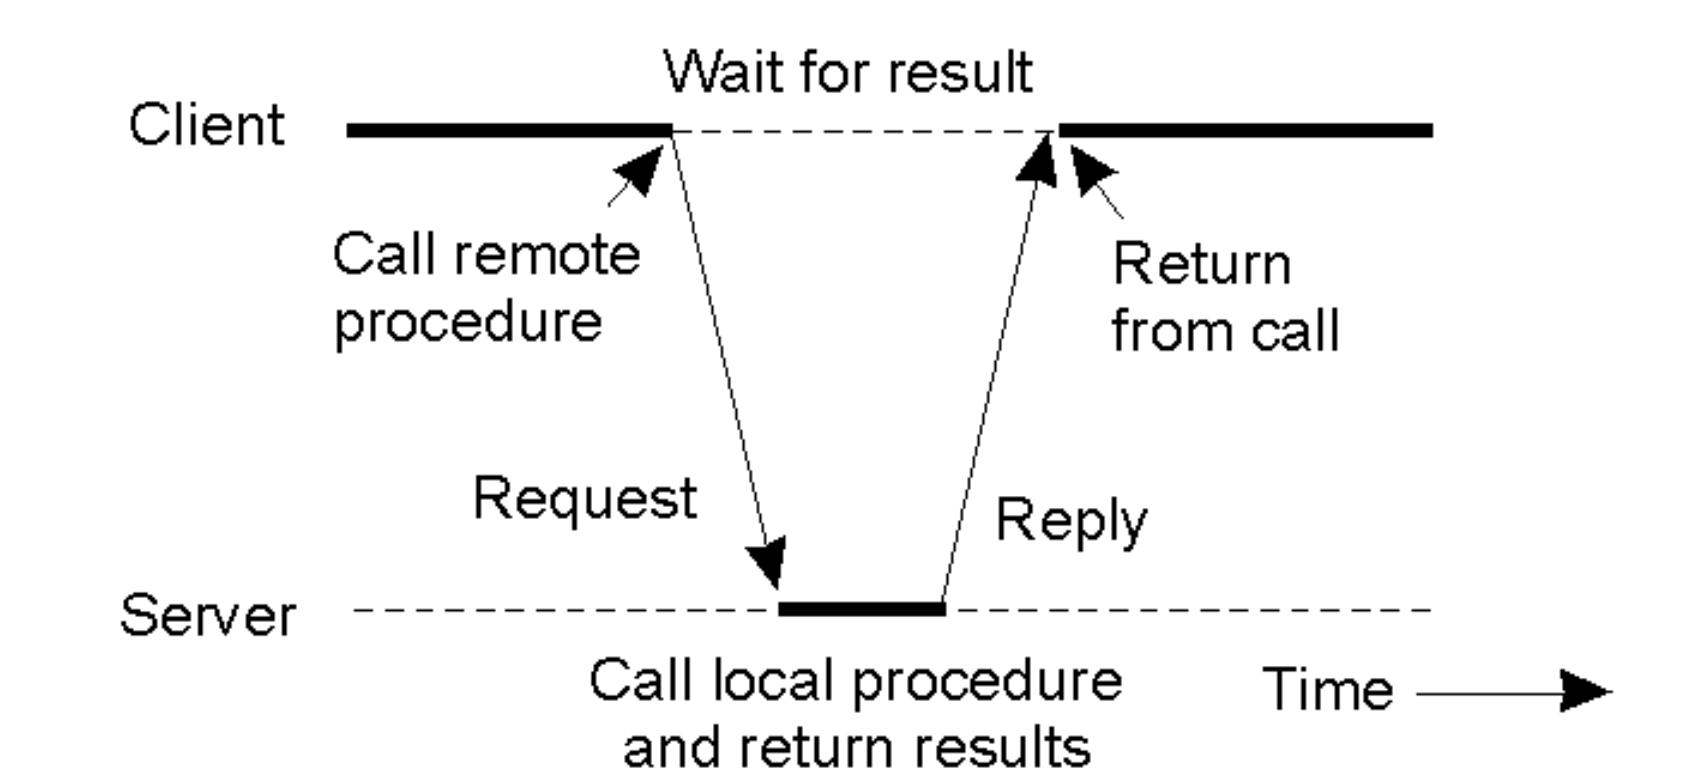
\includegraphics[scale=0.35]{rpc_blocking.png}
\caption{RPC as a blocking call}
\end{figure}

\begin{figure}[!h]
\centering
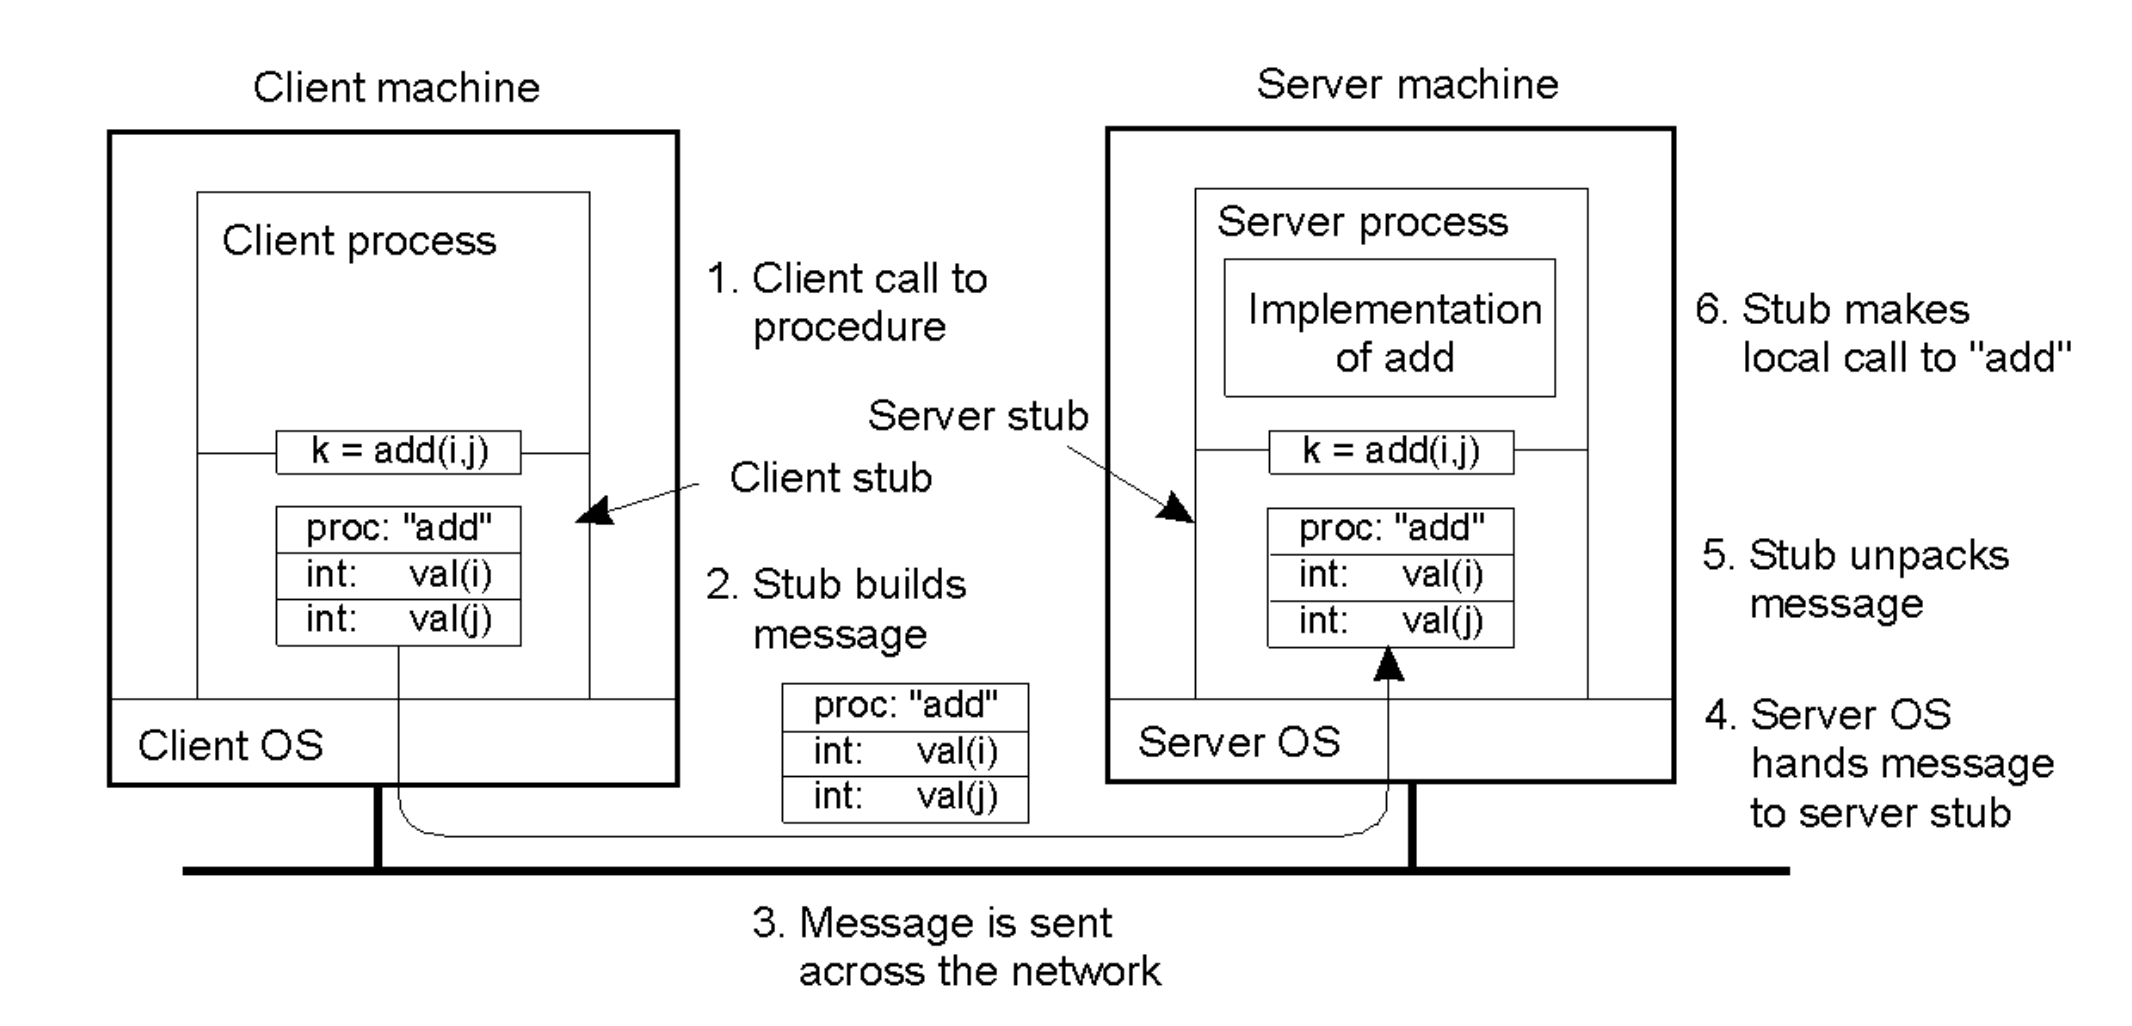
\includegraphics[scale=0.5]{rpc_flow.png}
\caption{RPC - an example}
\end{figure}

\textbf{Q: If you have two remote procedures and both are called add(), how is the client is going to know where the server is at?}
\\{Instructor: That is always the first problem in any distributed application that how do you know where the server is? One way is to hardcode the IP address which is not the best method. Ideally what would happen is when a server process starts up, it would register itself with a naming service saying I am a server and I am going to expose the add() service. So when the client starts up, it is going to call the naming service saying I need a server that can provide me the add() service. The naming server will provide all the info about the required server to the client.}
\\\textbf{Q: Is the naming service handled by DNS?}
\\{Instructor: Typically this is not DNS. Its an IP lookup service and we will talk about it. There is an RPC service that runs for providing naming.}
\\\textbf{Q: How are we going to compile this?}
\\{Instructor: Short ans is you have to decide which functions are remote and invocable and then you create a special header file which generates extra code, syntax codes etc. (Later, the instructor gave a live example in class)}
\subsection{Parameter passing}
In local procedure calls, parameter passing happens either through call by value or call by reference and they use memory stack/pointers to achieve this. Global variables also have to be taken care of. Remote procedure calls use stubs and marshalling to make parameter passing look transparent (although typically, not all functionality is achieved). By default, most RPC systems will support call by value and not call by reference. The pointers in the local machine will not make sense if sent to a remote machine.
\\\textbf{Q: What if the argument you are passing in RPC is a graph which is a complex data structure?}
\\{Instructor: You will have to do kind of linearization of that data structure. You have to properly package the parameters of that graph. Its called marshalling and then at server side there will be de-marshalling.}

\subsection{Client and Server stubs}
Remote procedure calls are handled transparently at the client and server sides using stubs. They remove burden of explicitly programming remote procedure calls from the programmer. At the client side, the client makes a local procedure call to the client stub. Stub takes care of all parameter packing and sending them as messages. This process of packing arguments and sending messages is called marshalling. This stub code is automatically generated by a stub compiler using an interface definition language. At the server side, the server stub, automatically unmarshalls/unpacks the parameters and calls the relevant procedure. Stubs on both the sides are generated automatically by the RPC run-time system.

The steps involved in a RPC call is summarized below:\\
1. Client procedure calls client stub just like a local procedure call\\
2. Client stub prepares a message and calls the local OS to deliver it\\
3. Client OS sends message to the remote OS\\
4. Remote OS delivers the message to server stub\\
5. Remote stub unmarshalls parameters and calls server procedure\\
6. Server procedure does computation and returns result back to server stub\\
7. Server stub packs result in a message, calls server OS to deliver it back\\
8. Server OS responds back to client OS\\
9. Client OS gets message and delivers it to the client stub\\
10. Client stub unpacks result and returns it to client\\

\subsection{Marshalling}
Marshalling is a process during which one process packs all the arguments and information in a format understood by the other process. Marshalling is necessary because different architectures have different data representation formats. For example, Intel architectures use little endian representation while SPARC uses big endian representation. In order to make RPC operate seamlessly across architectures, marshalling is required. Therefore, by using a standard external data representation (XDR), it is possible to have a process on an Intel machine make an RPC call to a process on a SPARC machine. A related problem is that, if the data we're sending contains pointers, the remote machine cannot resolve the pointer without accessing the memory of client. Possible solutions to this problem include prohibiting use of pointers or resolving pointers over network when required (The latter is complicated and typically RPCs don't use pointers as arguments). 

\subsection{Binding}
Binding allows clients to easily locate servers and to query the services exposed by servers. A server can export its interface to a binding server (directory service as mentioned earlier) during initialization. This involves sending name, version, UID and handle or address to the binding server. The client then first sends a message to the binding server to import the server interface. The client can then use the handle to communicate with the server. The directory service keeps track of what services are running and where the functions are exposed. Binder can also do load balancing by if a particular server is overloaded and the same interface is exported by another server. Binding is usually done at runtime.\\
Related issues are:\\
1. Exporting and importing interfaces adds more overhead\\
2. A single binding server can be a bottleneck; need replicated binders if necessary\\
\\\textbf{Q: How do you locate the binder?}
\\{Instructor: You can get it by broadcasting by sending a broadcast message on LAN saying is there a lookup server/binder running. If it is you will get the information where. Or, your system administrator can configure it and send that information to you. }
\\\textbf{Q: When a server registers itself with the binder, how will the binder know if that server is still running?}
\\{Instructor: Its an implementation issue. So your binder can choose different methods like the registration can be kept valid for certain period of time and it has to renewed or send  heartbeat messages etc. By default, the entries stay in the binder. But if you keep it there forever, it not going to work because the server is not going to run forever. So there has to be a method to deal with it and make sure the entries are valid.}
\\\textbf{Q: Can you pass some arguments where some parts of it are pointers?}
\\{Instructor: You should typically not send anything which has pointer in it.}
\\\textbf{Following Questions were asked for the live example code.}
\\\textbf{Q: The server code puts up extra arguments. What are those?}
\\{Instructor: That is a convention that you need these arguments. But you don't actually have to do anything with them. Its passed so that you can send some information back to the stub}
\\\textbf{Q: If you are running this program on a distributed machine which files would be on which machine?}
\\{Instructor: If you are writing client and server then you write the code. Then compile it and after compilation you will get the client and server binaries which can run on different machines.}
\\\textbf{Q: Where is the add.x needed?}
\\{Instructor: Its needed during compilation. Once you have binaries add.x is not needed.}

\subsection{Failure semantics}
Failures need to be appropriately dealt with. What if a client is blocked, waiting for a server and server dies? What if network is bad? (To deal with bad network we can use re-transmission techniques but must be careful and make sure that the requests are idempotent in nature. Think of a banking server example and client re-transmits multiple "deposit \$ in my account" requests). We now classify the types of errors a distributed system using RPCs can experience:
\begin{itemize}
  \item \textbf{{Client unable to locate server }} : Return error to the client.
  \item \textbf{{Lost request messages}} : Use timeout mechanisms. This can be detected if no response is obtained after a certain amount of time.
  \item \textbf{{Lost reply messages}} : Use timeout to detect. Make operation idempotent - triggering the operation multiple times will yield the same result. Alternatively, sequence numbers can be used and re-transmissions can be explicitly marked to let the server know. The code should be idempotent and this has to be done by the programmer.
  \item \textbf{{Server failures}} : Did the server fail before or after executing the operation?\\ At least once: The operation is executed at least once. Operation is retried until a response is received.\\ At most once: The operation is either executed exactly once, or not executed at all. \\Exactly once: The desirable choice ideally but difficult in practice.

  \item \textbf{{Client failures}} : When server is executing an RPC and client dies, it is called as an orphan RPC\\
    Extermination: In extermination, client logs requests at the client stub (i.e., detect client crashes) and explicitly kill orphans.\\
    Reincarnation: When client reboots, it sends a new epoch number to the server. The server then deletes computations of old epoch. A variation, called Gentle Reincarnation tries to locate the owner first and delete computations only if no owner was found.\\
    Expiration: Each RPC is given a fixed quantum T. Computation is aborted after T. Clients have to explicitly request extensions for computations taking longer than T.
\end{itemize}

\subsection{Implementation issues}
\begin{itemize}
  \item {Choice of protocol}: Choice of protocol greatly affects the choice of communication. This decision depend on packet size restrictions of the available protocol, whether flow control is required, reliability vs speed tradeoff, etc. If TCP is used, transmission losses needn't be taken care of RPC designer.
  \item {Overhead of copying}: Message has to be copied multiple times - this adds to overhead. At least 2 copies are required. This can go up to 7 copies per message (Eg- Stack in stub - Message Buffer in Stub - kernel - NIC's buffer - physical medium - Server's NIC - Server kernel - Server stub. 7 copies). Although, copying mechanisms like scatter-gather operations (which pass pointers within a system as much as possible) do exist which reduce overhead to an extent.
\end{itemize}

\begin{figure}[h]
\centering
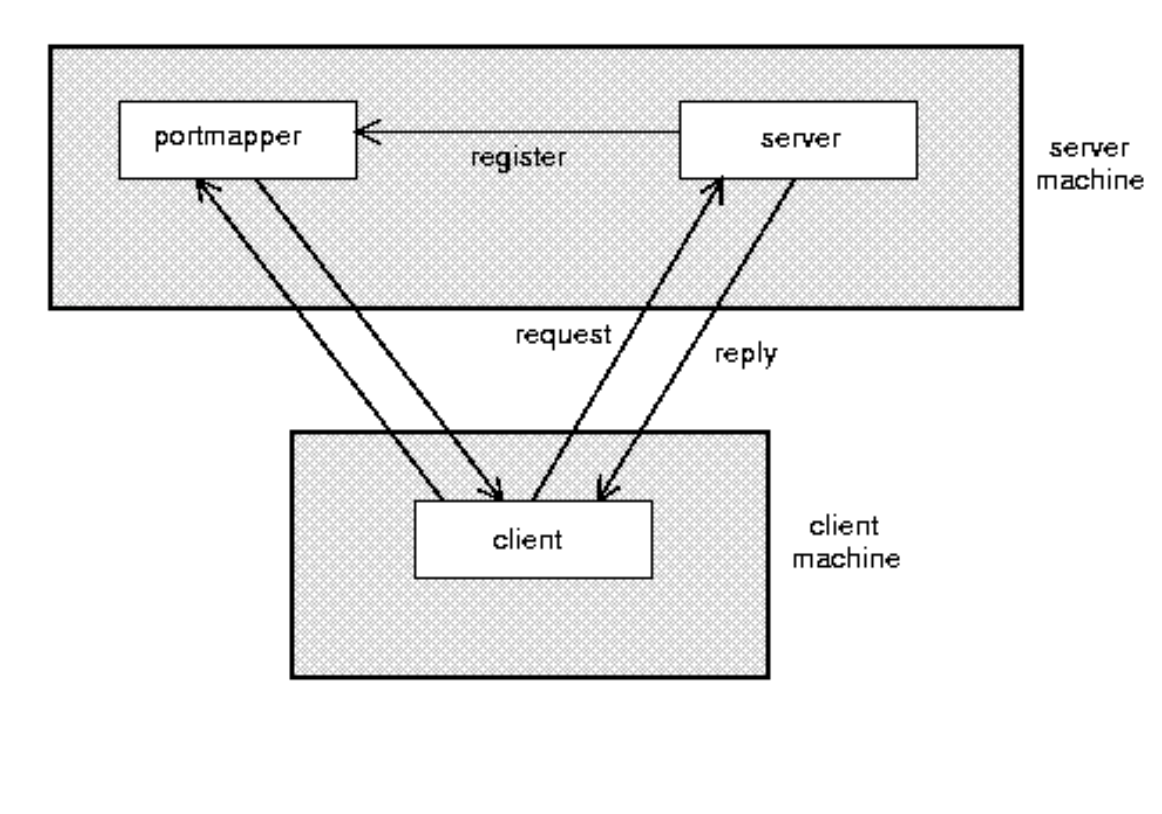
\includegraphics[scale=0.5]{port_mapper.png}
\caption{Port mapper}
\end{figure}

\subsection{Case study: SUNRPC (from previous notes)}
SUNRPC is one of the most widely used RPC mechanism. Either TCP or UDP can be used as the underlying protocol. During marshalling, multiple arguments are packed into a single structure. It uses SUN's external data representation (XDR) to provide compatibility across different architectures. This internally uses big endian ordering. SUNRPC is used by NFS (network file system).

SUNRPC's binder is called port mapper. When a server starts up, it creates a port and registers its service with the local port mapper (using svc\_register). On client start up, it locates server port using (clnt\_create) and then can use services offered by the server.



SUN's RPC package also includes an RPC compiler that automatically generates stubs for client and server. The programmer has to write client code, server code and a .x file (this interface specification file contains interfaces of all RPC messages). Then RPC compiler creates four files: server stub, client stub, a header file and the XDR code. The client application + client stub + header can then be sent to C compiler creating the client binary and the server application + server stub + XDR together create the server binary. When both these binaries are run, client-server communication is possible with RPCs.

\end{document}
